\section{Revert}

The program can be reverted to the last saved state by using revert. The button for which is located in the edit menu.
The revert functionality is only present if there are unsaved changes.
Revert will ask for conformation before reverting because once the revert has been applied, any information not saved will be permanently lost.
Revert will also ask if you want to save changes as a new file before reverting.
\newline\newline


\begin{figure}[H]
\centering
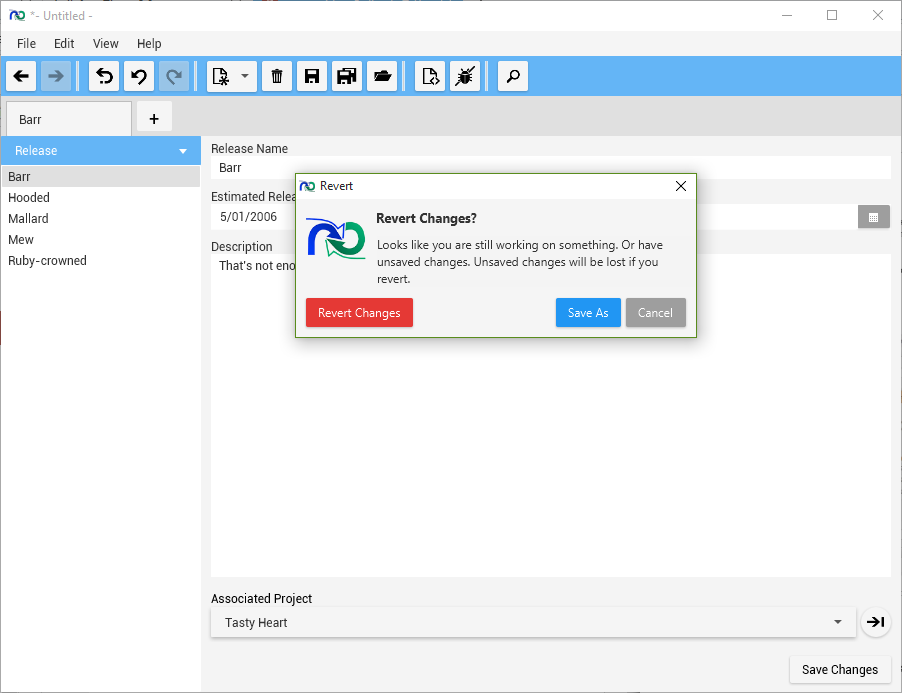
\includegraphics[width=\textwidth]{images/screenshots/revert1.PNG}
\caption{Reverting a change}
\label{fig:revert}
\end{figure}